This section outlines benchmark models for both background from the QCD and for new
physics signals that encapsulated in the models chosen: Strings, graviton and QBH.
Full Run 2 data are used to produce EXOT2 skimmed samples used in this analysis~\cite{ATLAS:Exot2Derivation}.

\subsubsection{QCD background}
\label{qcdsamps}

QCD processes from the MC are simulated at LO and NLO in SM perturbative theory. Due to the large range in cross section of QCD sample~\cite{Marshall:2016630}, the samples are thus sliced based on the leading jet \pt,  to obtain comparable statistical precision across the jet \pt~range of interest.

% reweighting the underlying spectrum is described in Ref.~\cite{Marshall:2016630}.  


%\subsubsection{\Hprime}
%\label{sec:hprime}
%
%This analysis performs a model-independent search for two-gluon resonances at high \mjj spectrum, as the CCD background is dominated by valence quark scattering, gluon tagging in this case could be effective. 
%
%The simulated SU(3) singlet scalar that decay via \pythia8 with the A14 set of tuned 
%parameters is used in this analysis\footnote{See \url{https://its.cern.ch/jira/browse/ATLMCPROD-6155}.}. The HiggsBSM:gg2H2, where set the singlet scalar as H2 particle and has Particle Data Group ID 35. Such H2 particle is set to decay to gluons and has a narrow resonances width of 0.1 GeV as the physical width is 
%model-dependent but constrained by the detector resolution.
%
%The benchmark signals used vary in their underlying physics motivation, but also in the resulting shape of the signal \mjj distribution. The peaks of signal shape are set for various mass points as shown in Figure~\ref{fig:shape_Hprime}, the distributions are normalized to unity and thus the differences in peak amplitudes are not the changes in cross section.
%
%\begin{figure}[htb]
%\centering
%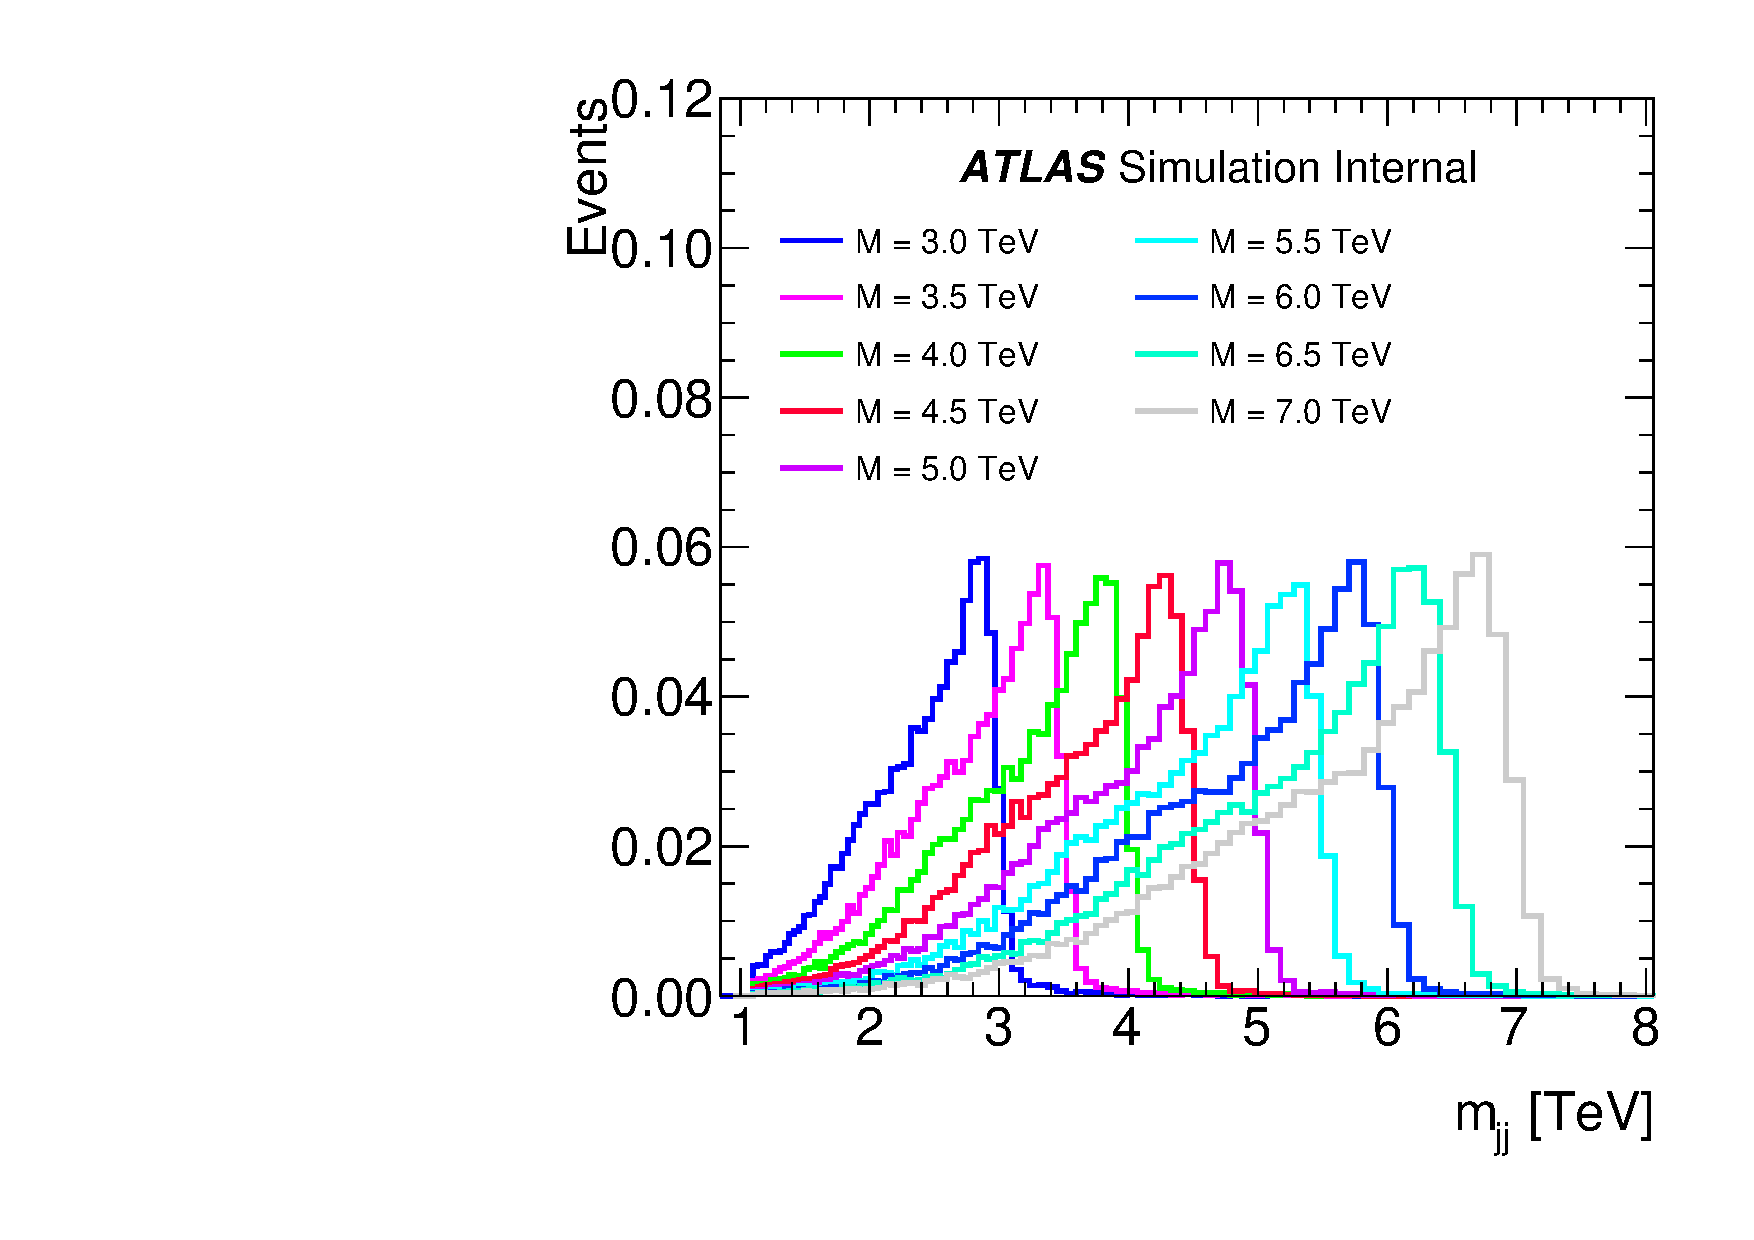
\includegraphics[width=0.65\textwidth]{fig/benchmark_signals/SignalShape-Hprime.pdf}
%\caption{Signal shapes for the \Hprime~signal at different mass points.}
%\label{fig:shape_Hprime}
%\end{figure}
%\FloatBarrier

%\subsubsection{String}
%\label{sec:string} % uncomment if label used. 
%As the SM has lots of well known problems such as the quadratically divergent corrections to the Higgs self-energy, supersymmetry theory offers a solution to it by fine-tuning the
%cancellation. The superstring theory, additional to the supersymmetry, can perform as a framework that unify theories from SM at TeV-scale to quantum gravity at Planck-scale. 
%
%The fundamental string scale is chosen to be within TeV scale, denotes as string mass-scale \Ms~. The string resonances could happen at masses $m_n = \sqrt{n} \Ms$, for $n = 1, 2, 3, \ldots$, where the resonance consist of the Regge excitations of quark, gluon, as well as the colour singlet that lives on the QCD stack of branes. In total, five string scales \Ms range from 7.0~TeV to 9.0~TeV, in steps of 0.5~TeV are generated for string-resonance samples~\cite{Anchordoqui:2008hi}. The lower limits of mass $M_\mathrm{min}$ provided in the generator are shown in Table~\ref{tab1}, together with the resulting cross section of the string samples.
%
%Searches for string resonances have been done in previous dijet mass spectra~\cite{ATLAS:2012pu,Chatrchyan:2011ns,CMS:2012yf,Khachatryan:2015sja,Khachatryan:2015dcf,Sirunyan:2018xlo}. It is worth noting that the string resonance searches mentioned in these references have limitations in terms of model constraints and the clarity of the methodologies used. 
%
%
%%The string-resonance widths have been calculated in Ref~\cite{Anchordoqui:2008hi}. 
%
%\begin{table}[htb]
%\begin{center}
%\begin{tabular}{ccc}
%\toprule
%%[-2ex]
%\Ms & $M_\mathrm{min}$ & Cross section\\
%{[TeV]} & {[TeV]} & {[fb]}\\ 
%\midrule 
%\num{7.0} & \num{6.06} & \num{7.09E+0}\\
%\num{7.5} & \num{6.60} & \num{1.86E+0}\\
%\num{8.0} & \num{7.14} & \num{4.56E-1}\\
%\num{8.5} & \num{7.60} & \num{1.00E-1}\\
%\num{9.0} & \num{8.05} & \num{1.99E-2}\\
%\bottomrule
%\end{tabular}
%\end{center}
%\caption{MC string-resonance samples with string scale \Ms,
%minimum mass $M_\mathrm{min}$, and cross section.} 
%\label{tab1}
%\end{table}
%
%The first $(n=1)$ resonant pole is considered in this study. The widths of string-resonances have been calculated in this Ref~\cite{Anchordoqui:2008hi}. As the string resonances have long Breit-Wigner tails, the PDFs at low-$x$ (low mass) can significantly enhance the tail. In this study, the low-mass tail is truncated since only narrow-resonance structure in \mjj spectrum is interesting to this analysis. In the range $7.0 \leq \Ms \leq 8.0$~TeV, the truncation is done at the minimum value in the differential cross section on the lower-mass side of the \Ms peak, results in around 95\% of the area under the Breit-Wigner curve. In the range $7.0 \leq \Ms \leq 8.0$~TeV, the truncation is done at at a lower-mass point that covers 95\% of the area under the Breit-Wigner curve.
%
%The distribution of signal peak at different mass points is shown in Figure~\ref{fig:shape_strings}, the distributions are normalized to unity and thus the differences in peak amplitudes are not the changes in cross section.
%
%\begin{figure}[htb]
%\centering
%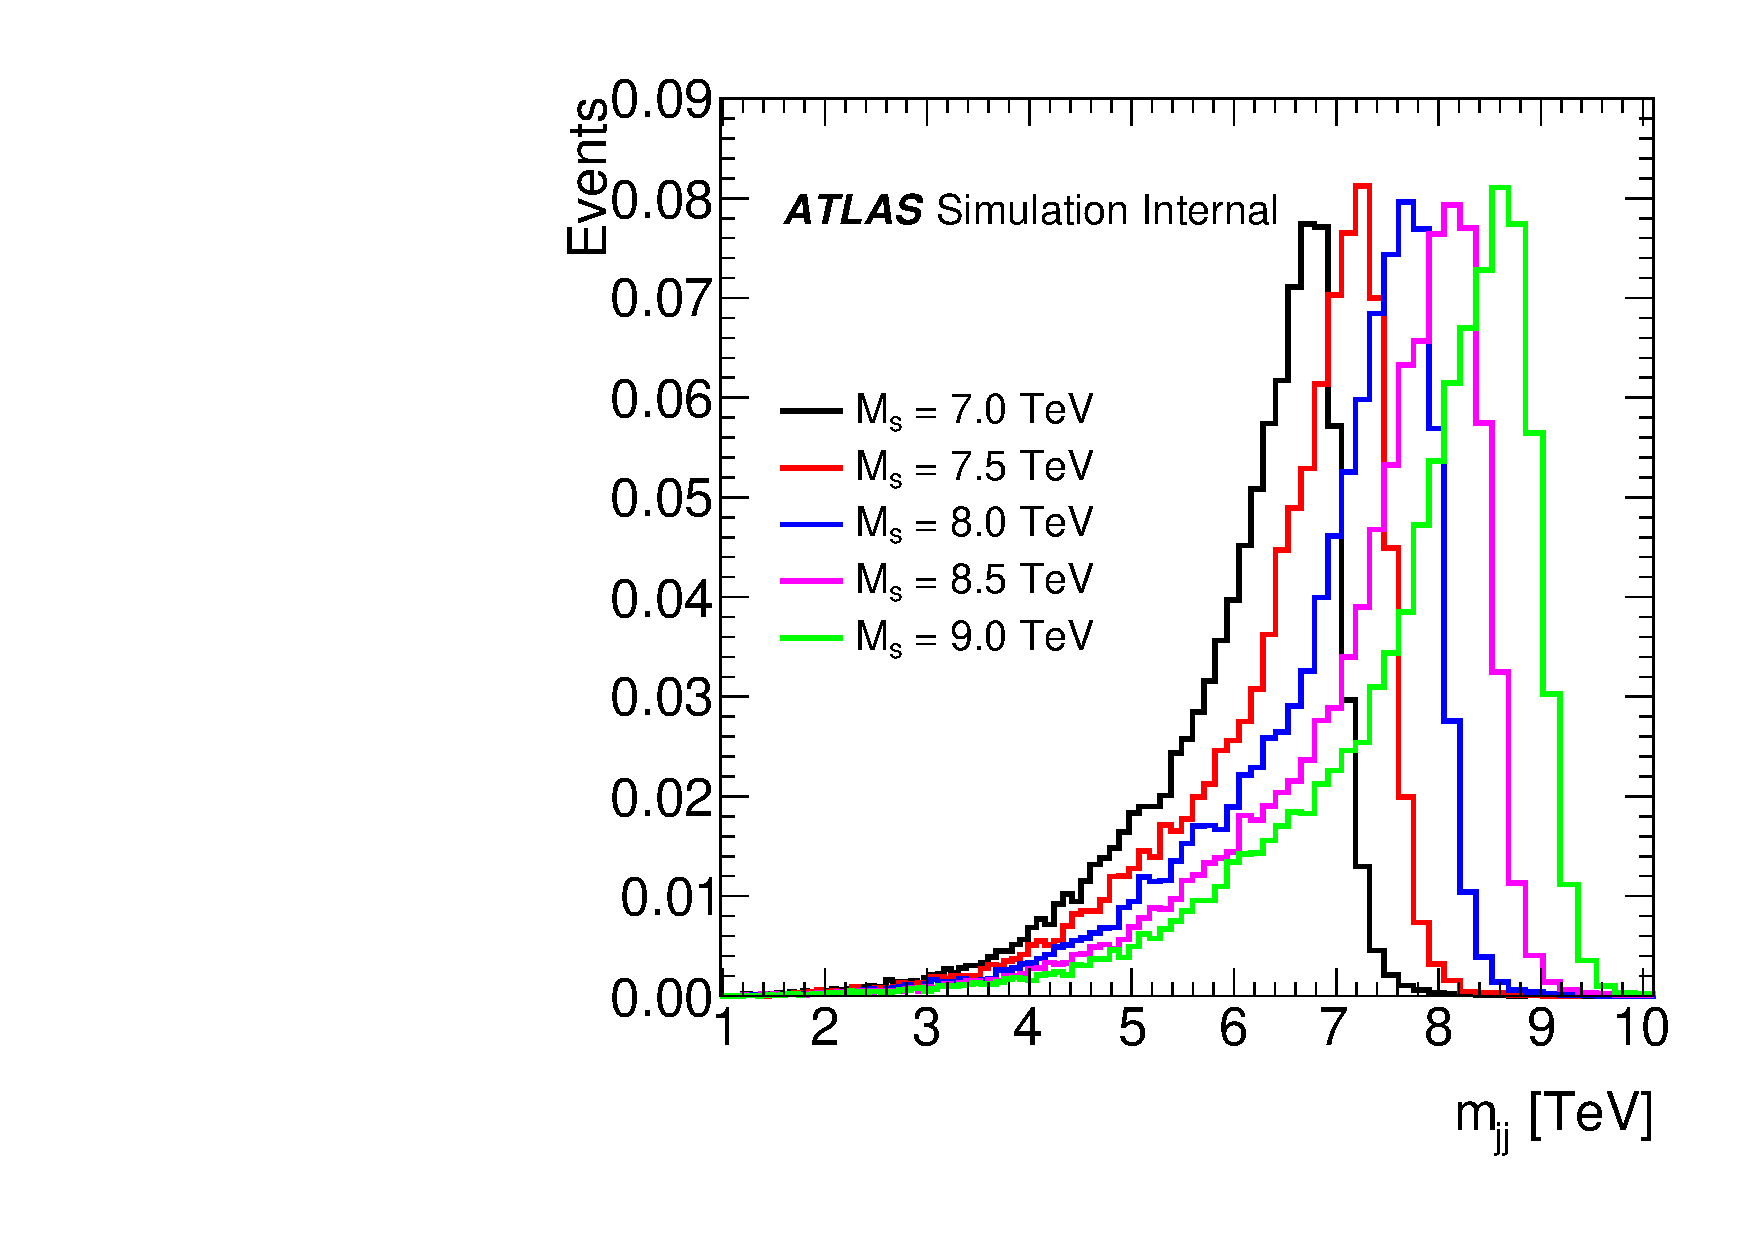
\includegraphics[width=0.65\textwidth]{fig/benchmark_signals/SignalShape-strings.pdf}
%\caption{Signal shapes for the String signal.}
%\label{fig:shape_strings}
%\end{figure}
%
%
%There are five possible $2\to 2$ subprocesses from string resonances are simulated. with the cross section for each subprocess vary as a function of \Ms\ shown in Table~\ref{tab2}. The dominate subprocess across the \Ms\ values is considered to be $gq\to gq$, which contributes around 81-87\% of the total cross section. The rest of subprocesses: $qq\to qq$, $\bar{q}\bar{q}\to \bar{q}\bar{q}$, and $q\bar{q}\to
%q\bar{q}$ are model dependent and thus do not included in this analysis. 
%
%
%\begin{table}[htb]
%\begin{center}
%\begin{tabular}{crrrrr}\toprule
%Subprocess             & \multicolumn{5}{c}{\Ms\ {[TeV]}}\\
%& \multicolumn{1}{c}{7.0} & \multicolumn{1}{c}{7.5} &
%\multicolumn{1}{c}{8.0} & \multicolumn{1}{c}{8.5} &
%\multicolumn{1}{c}{9.0}\\ 
%\midrule
%$gg\to gg$             & 11.4\% &  9.5\% &  8.2\% &  7.2\% &  5.1\%\\
%$gg\to q\bar{q}$       &  0.3\% &  0.3\% &  0.2\% &  0.2\% &  0.2\%\\
%$gq\to gq$             & 81.4\% & 83.1\% & 84.6\% & 85.5\% & 87.6\%\\
%$g\bar{q}\to g\bar{q}$ &  0.7\% &  0.6\% &  0.5\% &  0.5\% &  0.5\%\\
%$q\bar{q}\to gg$       &  6.3\% &  6.5\% &  6.5\% &  6.5\% &  6.7\%\\
%\bottomrule
%\end{tabular}
%\end{center}
%\caption{String-resonance subprocesses and their relative contributions
%to the total cross section at each string scales \Ms.
%The statistics are based on samples of 66000 events.}
%\label{tab2}
%\end{table}
%
%For generating string samples, the MC event
%generator \str~1.00~\cite{Vakilipourtakalou:2018pfo} 
%with interfaced to \pythia8.240~\cite{Sjostrand:2014zea} for parton shower modelling is used, together with the A14 tune.%~\cite{ATL-PHYS-PUB-2014-021}.
%The CTEQ6L1~\cite{Pumplin:2002vw} PDF set at the LO is used for the parton shower and the hard-scattering process. The decaying processes is simulated using the EvtGen~1.6.0 program.~\cite{Lange:2001uf}.
%
%The effect from pile-up is simulated by overlaying the MC inelastic $pp$
%events generated with \pythia8.186 with a PDF set of NNPDF2.3 at LO and the A3~\cite{ATL-PHYS-PUB-2016-017}  tune over the original hard-scattering events. 
%
%
%\FloatBarrier

\subsubsection{Kaluza-Klein Graviton}
\label{sec:kkgraviton}

For the RS KK graviton samples considered in this study, we focus on $k/\overline{M}_{PI} = 0.2$. These samples encompass both gluon-gluon and quark-quark initial states, with decays exclusively to gluons or bottom quarks.

The signal templates for the KK gravitons are generated with different mass values using the \pythia8 event generator. These simulations utilize the A14 tune and NNPDF2.3 PDF set.

Figure~\ref{fig:Ggg} shows the Graviton to gg invariant mass distribution for the considered mass points.

\begin{figure}[!h]
	\centering
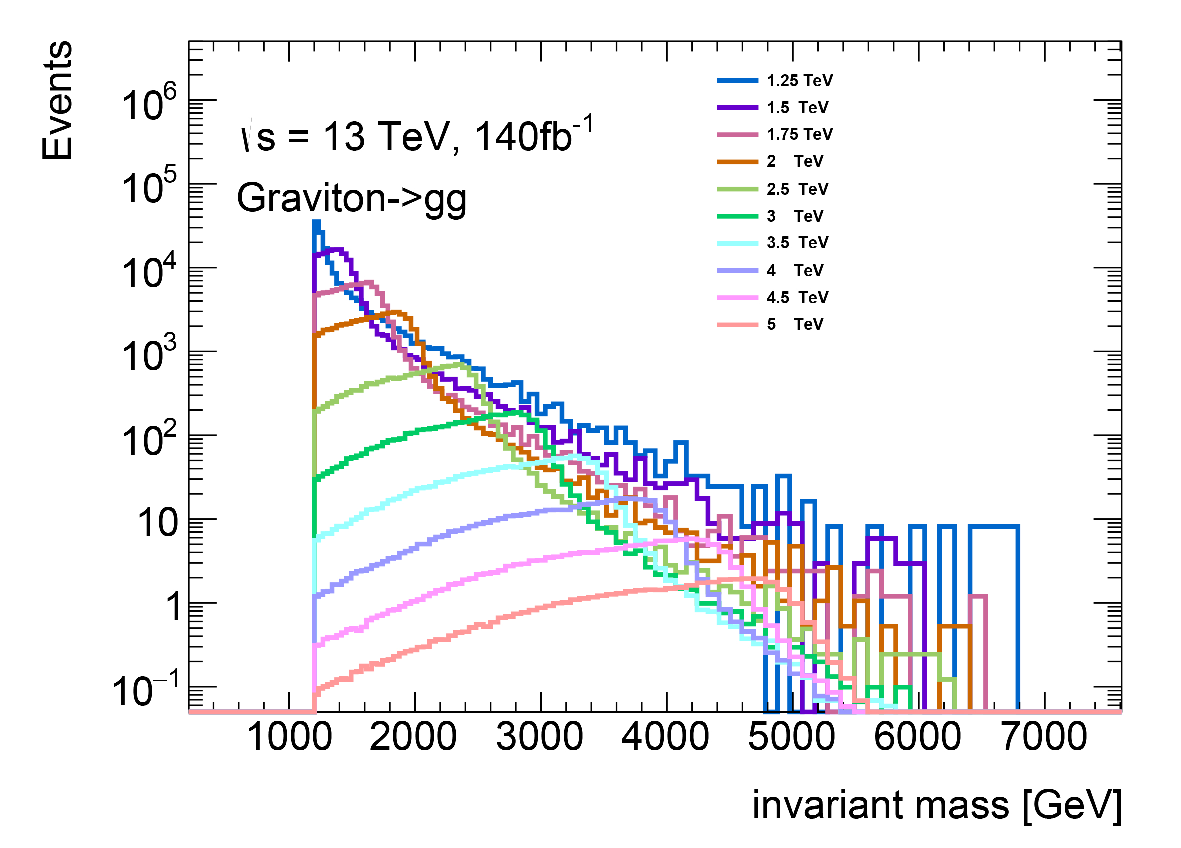
\includegraphics[width=0.75\textwidth]{fig/benchmark_signals/Ggg_mjj.pdf}
	\caption{(a) Invariant mass distribution for the Graviton to gg samples
		\label{fig:Ggg}
	}
\end{figure}

\begin{comment}


\subsubsection{Excited quarks}
%\label{sec:qstar}

We are using an excited quark model for performing limits comparison with the
previous iteration of the analysis.

Excited quark \qstar production and subsequent decay to
quarks and gluons via gauge interactions has been
used as a common benchmark for the dijet mass resonance
search~\cite{EXOT-2010-01,EXOT-2010-02,EXOT-2010-07,EXOT-2011-07,EXOT-2013-11,EXOT-2016-21},
and it is described in detail in Refs~\cite{Baur:1987ga,Baur:1989kv}.
The $qg\to$ \qstar production model~\cite{Baur:1987ga,Baur:1989kv} is used,
with the assumption of spin 1/2 and quark-like SM coupling constants.
The compositeness scale $\Lambda$ is set to the \qstar~mass.

The excited quark signal templates are generated for different mass values(Appendix~\ref{section:MCqStarSamples}) with the \Pythia~8 event generator~\cite{pythia8},
using the A14 tune~\cite{A14tune} and NNPDF2.3 PDF set~\cite{Carrazza:2013axa}. Both light flavor ($u$,$d$,$s$) and heavy flavor ($c$,$b$) quarks are taken into account in
the event generation.
After a basic selection, no duplicate events have been identified.
All samples are fully simulated using \Geant.

Figures~\ref{fig:signal_xsec} and~\ref{fig:acc} show the cross sections and
acceptances as a function of the signal mass point.  
The acceptance shown for the \qstar model for 13~\TeV~center-of-mass energies 
uses the full resonance analysis selection (Section~\ref{sec:event_selection}).
The interpolation between points is a straight line therefore the
acceptance between mass of 1~\TeV~and mass of 2~\TeV~is not an accurate representation
of what the acceptance of a mass 1.5~\TeV~sample would be.  The
interpolation is not used but drawn to help guide the eye.

\begin{figure}[!htb]
  \centering
  \subfigure[Cross section]{ \label{fig:signal_xsec} 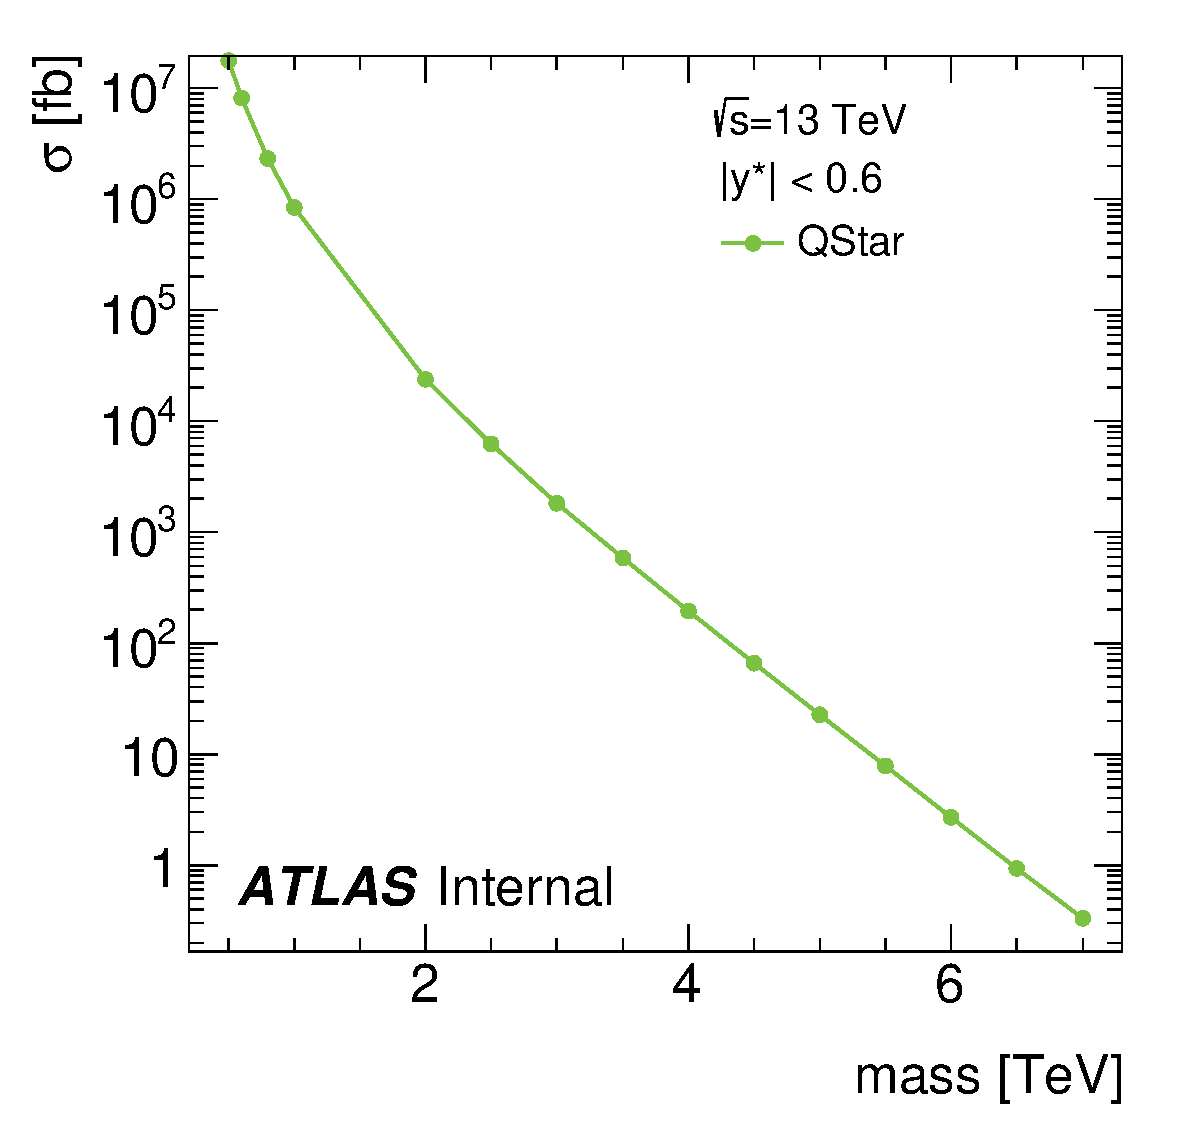
\includegraphics[width=0.48\textwidth]{figures/benchmark_signals/CrossSections_QStar_log} }
  \subfigure[Acceptance]{ \label{fig:acc} 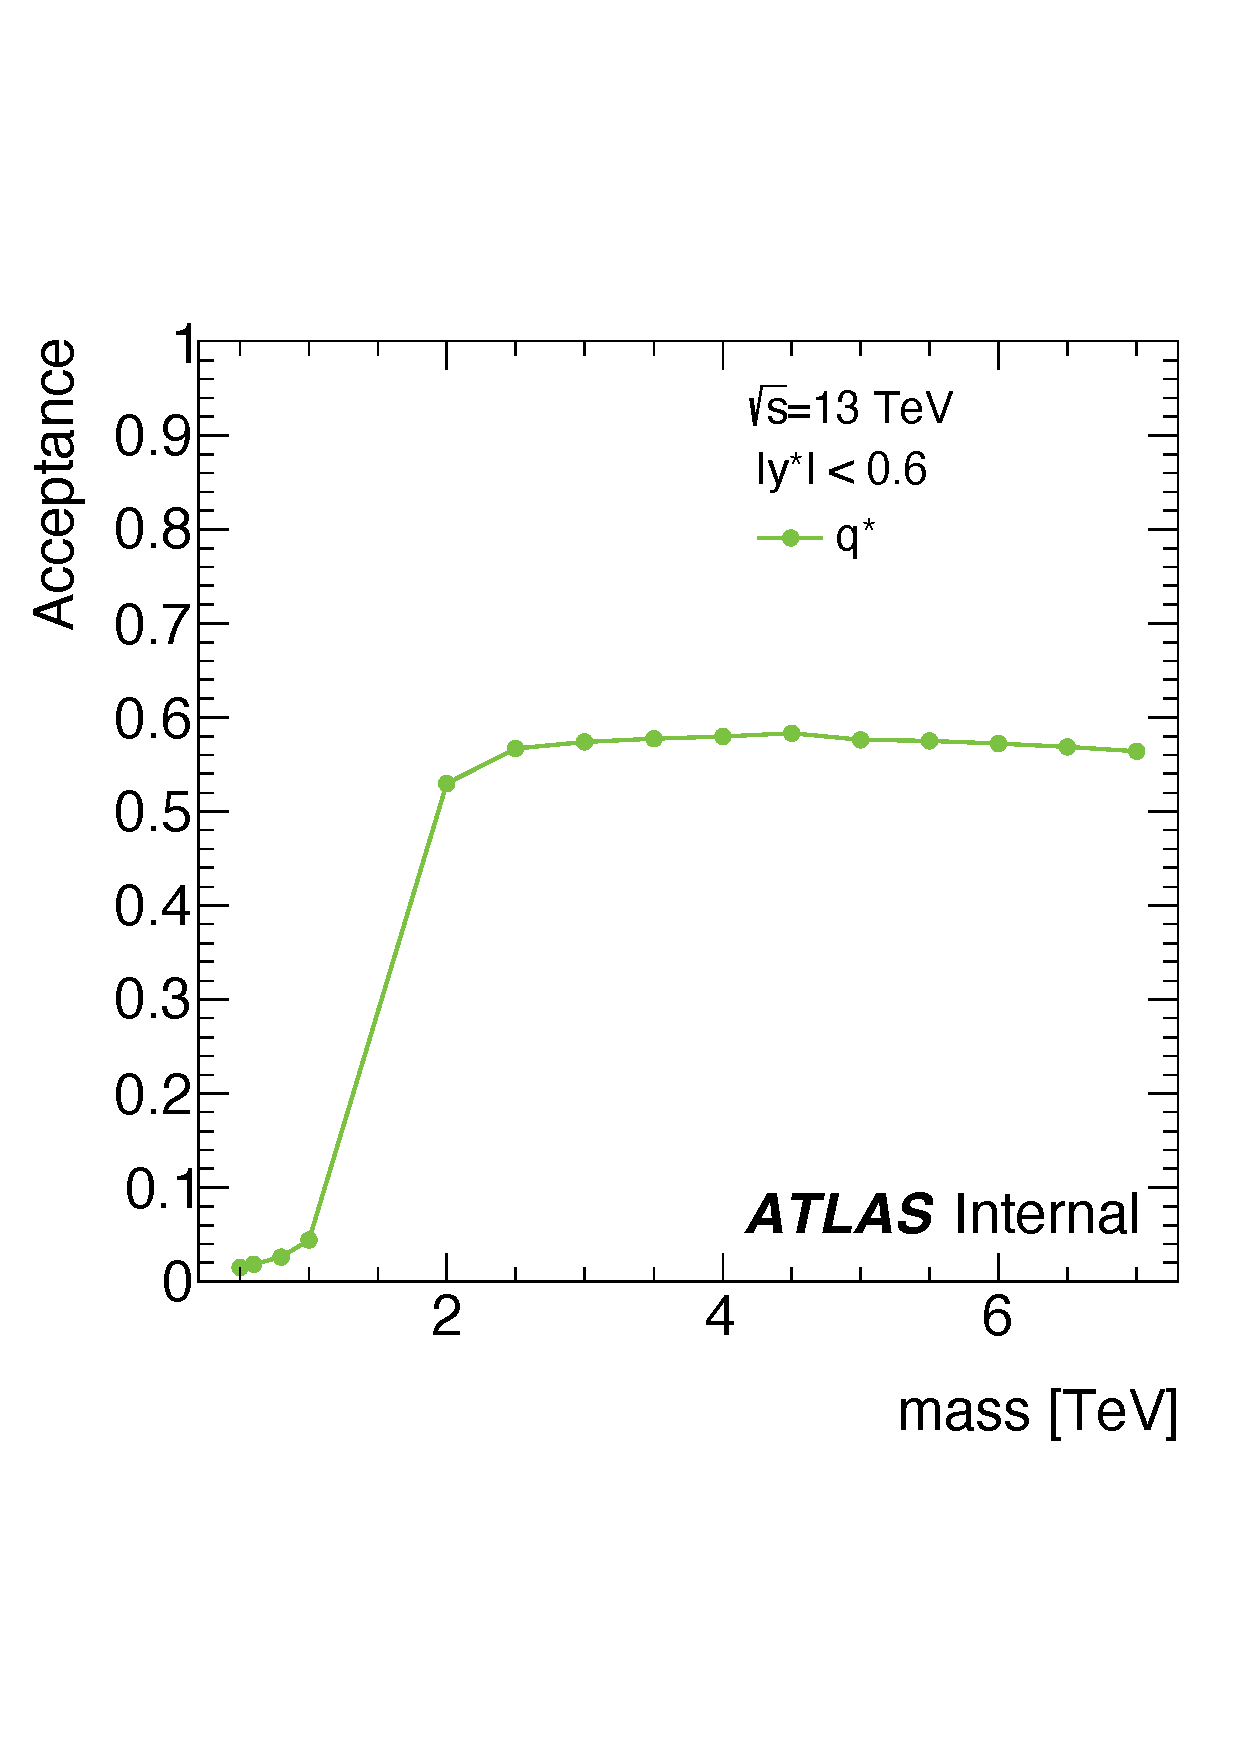
\includegraphics[width=0.48\textwidth]{figures/benchmark_signals/Acceptances_QStar} }
  \caption{(a) Cross section and (b) acceptance for the 
  light-flavored \qstar model for 13~\TeV~center-of-mass energies using the full resonance
  analysis selection (Section~\ref{sec:event_selection}).}
\end{figure}

\FloatBarrier
\end{comment}
\subsubsection{Quantum Black Hole}
%\label{sec:QBH} % uncomment if label used. 
%\todo{Do QBH decay to quarks or gluons, is there increased sensitivity or not} 
In our study, we employ the QBH model for the purpose of comparing limits with the previous iteration of the analysis. The feasibility of producing QBHs at the LHC is contingent upon the presence of sufficiently large extra dimensions within the universe~\cite{RandallMeade}. This model posits that the energy scale of quantum gravity $M_{D}$, at which QBHs are generated, diminishes as the number of these large extra dimensions, denoted as $n$, increases. Consequently, a larger $n$ permits lower mass scales at which QBHs can be formed.

Two-body isotropic final state is expected by the QBH decay at the LHC, where the $M_D$ energy threshold could be reached~\cite{Feng:2004}. Therefore the quantum gravitational effects can be probed by searches on \mjj spectrum. To simulate events involving quantum black holes with $n=6$, we utilize the \BlackMax~\cite{Dai:2007ki} MC generator. This MC generator facilitates the simulation of QBH events within the $n=6$ framework。

\subsubsection{Gaussian resonances}

A model-independent signal as Gaussian~\cite{lukacs1942characterization} are used to expand the sensitivity of the search to new signals that may be detectable with this analysis but not currently theoretically described. Besides, a model-independent signal could help to evaluate and compare the strength of different analyses without bias, as the case where specific models are applied and leads less sensitive to the search.

Therefore, model-independent fit function tests are produced based on model-independent signal resonances. Because this analysis is sensitive to the shape of resonance, specific models with different shapes would influence the results strongly. In general, a model-independent signal is a good feature of the analysis which verify the ability to distinguish different signal models, although the model-independent limits are still influenced by the shape of the resonance in an implicit way. The motivation to choose a Gaussian resonance as a proxy is the fact that it is similar to the `average' signal with specific width. Besides, the shape of reconstructed jet \pt~of any realistic signal without very specific model is produced approximately as a Gaussian resonance, without applied JER. Hence it it straightforward to use Gaussian resonances to represent any realistic resonance.

The general form of Gaussian distribution is:

\begin{equation}
	f(x)=\frac{1}{\sigma \sqrt{2 \pi}} e^{-\frac{1}{2}\left(\frac{x-\mu}{\sigma}\right)^2}
\end{equation}
where the parameter $\mu$ is the mean or expectation of the distribution (and also its median and mode), while the parameter 
$\sigma$ is its standard deviation.

%%%%%%%%%%%%%%%%%%%%%%%%%%%%%%%%%%%%%%%%%%%%%%%%%%%%%%%%%%%%%%%%%%%%%%%%%%%%%%%%%
%
%\clearpage
%\subsubsection{Signal shapes in the various models}
%
%The shape of the signal peak for each mass point and each signal model, after the resonance selection cuts, are shown in Figure~\ref{fig:showallshapes}. Each template is normalised to 1, and therefore differences in peak amplitude are indicative of a broadening or narrowing of the signal rather than of a change in cross section.
%\begin{figure}[!htb]
%\centering
%\subfigure[q* model]{\label{fig:resonance_templates_2500}
%               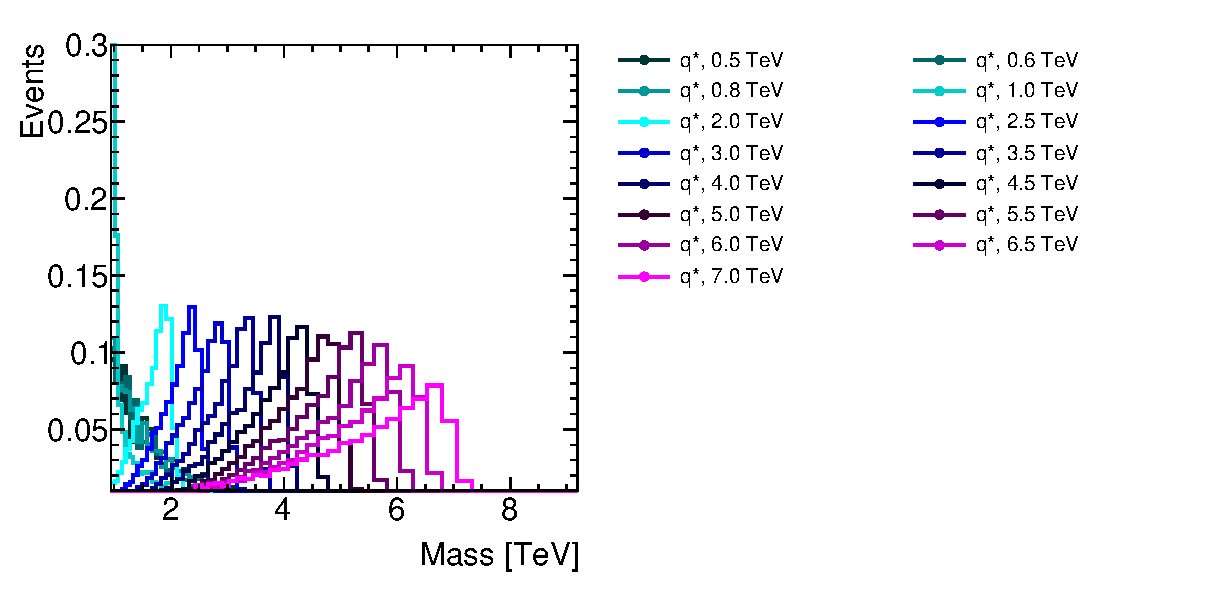
\includegraphics[height=0.25\textwidth]{figures/benchmark_signals/overlaidQStar_mjj_linear.eps}}
%\subfigure[\BlackMax\ model]{\label{fig:resonance_templates_4500}
%               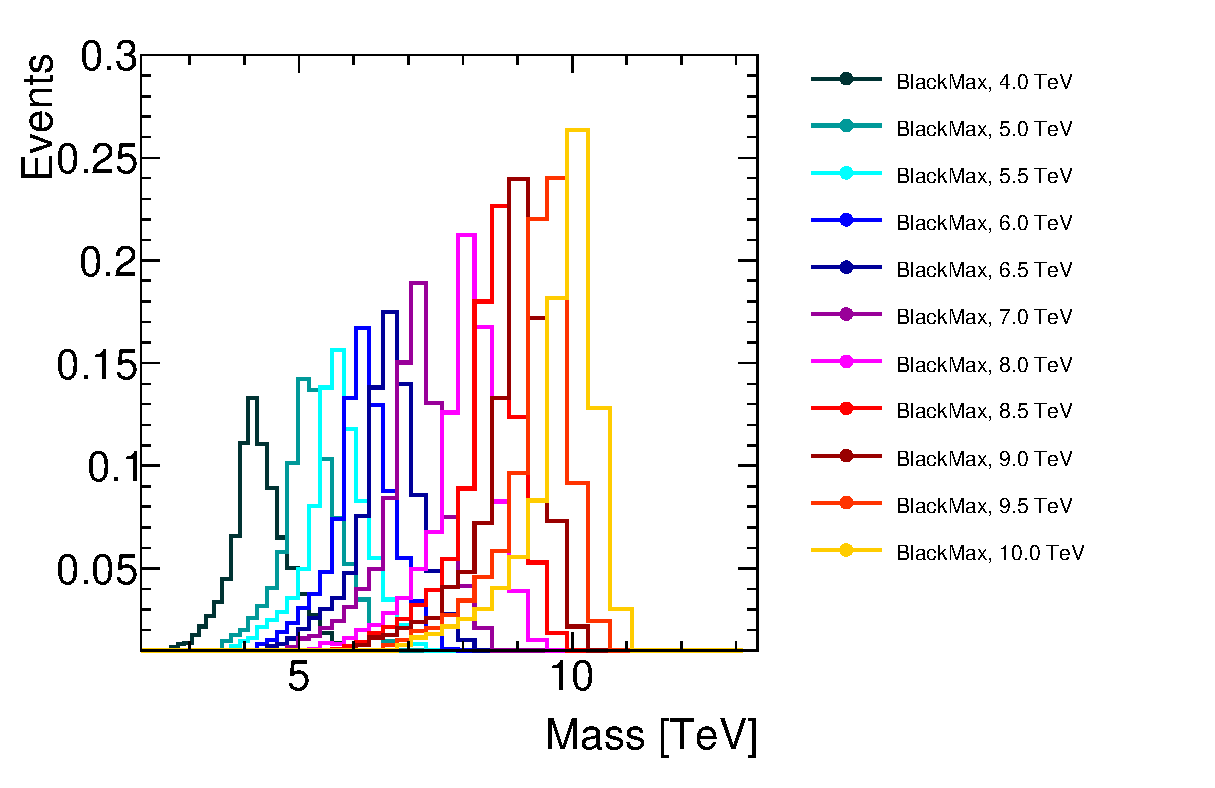
\includegraphics[height=0.25\textwidth]{figures/benchmark_signals/overlaidBlackMax_mjj_linear.eps}}
%\subfigure[\Wprime\ model]{\label{fig:resonance_tr_templates_2500}
%               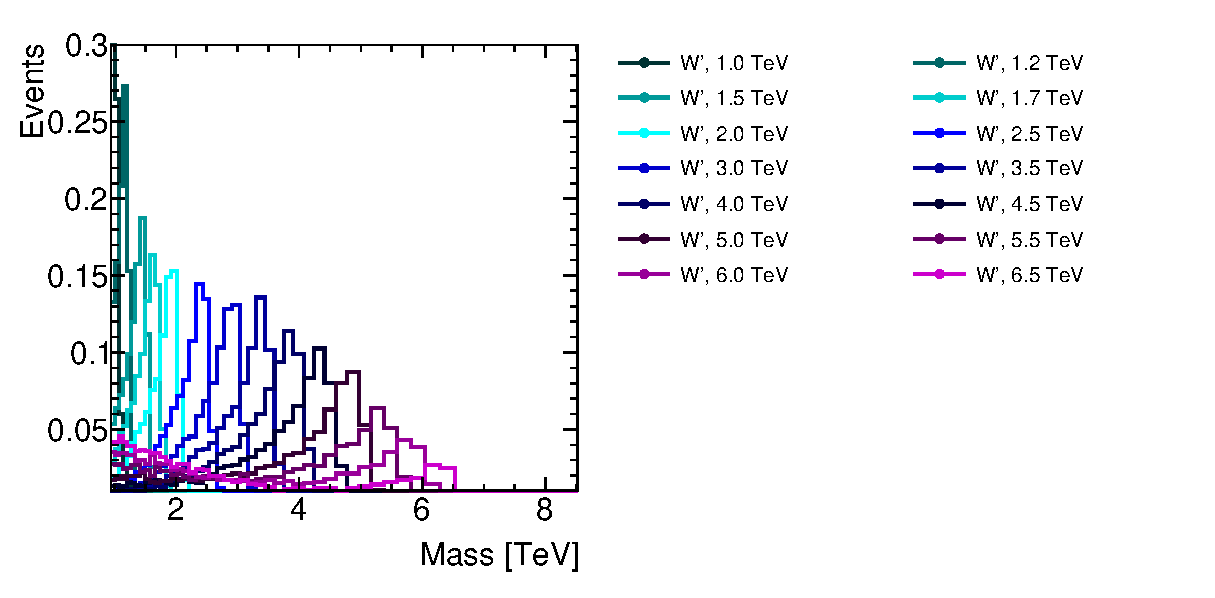
\includegraphics[height=0.25\textwidth]{figures/benchmark_signals/overlaidWPrime_mjj_linear.eps}}
%\subfigure[\Wstar\ model]{\label{fig:showallshapes}
%               \includegraphics[height=0.25\textwidth]{figures/Wstar/CrossAcceptance/MassesDist.pdf}}
%%\subfigure[4.5 TeV, truncated]{\label{fig:resonance_tr_templates_4500}
% %              \includegraphics[width=0.45\textwidth]{old_figures_2015/search_results/Resonance/Gaus_Comp/M4500_tr_comp.pdf}}
%\caption{Normalized \mjj\ templates at every mass point considered in the limit setting phasse for each of the resonant benchmark models. }
%
%\end{figure}
%

%This is demonstrated most clearly in Figure~\ref{fig:resonance_templates_shapes}, which shows overlaid reconstructed \mjj\ distributions for a selection of benchmark signals at the same mass point.
%The low-mass tail of \Wprime\ starts to become pronounced at higher masses, and the \qstar\ signal is also broadened. 
%In contrast to the previous two, 
%The detailed differences between the signal shapes become apparent in Figures~\ref{fig:resonance_tr_templates_4000} and \subref{fig:resonance_tr_templates_6500}, 
%which show the signal templates truncated at $\pm 20 \%$ of the generated mass. 
%This is the truncation recommended for recasting of the generic Gaussian observed limits set by this analysis into signals with peaked but non-Gaussian \mjj\ distributions. 
%The truncated distributions show that the \qstar\ signal distributions are shifted the most to lower \mjj\ of all signals, for both lower and higher masses. 
%% 
%% 
%\begin{figure}[!htb]
%\centering
%\subfigure[4.0 TeV]{\label{fig:resonance_templates_4000}
%               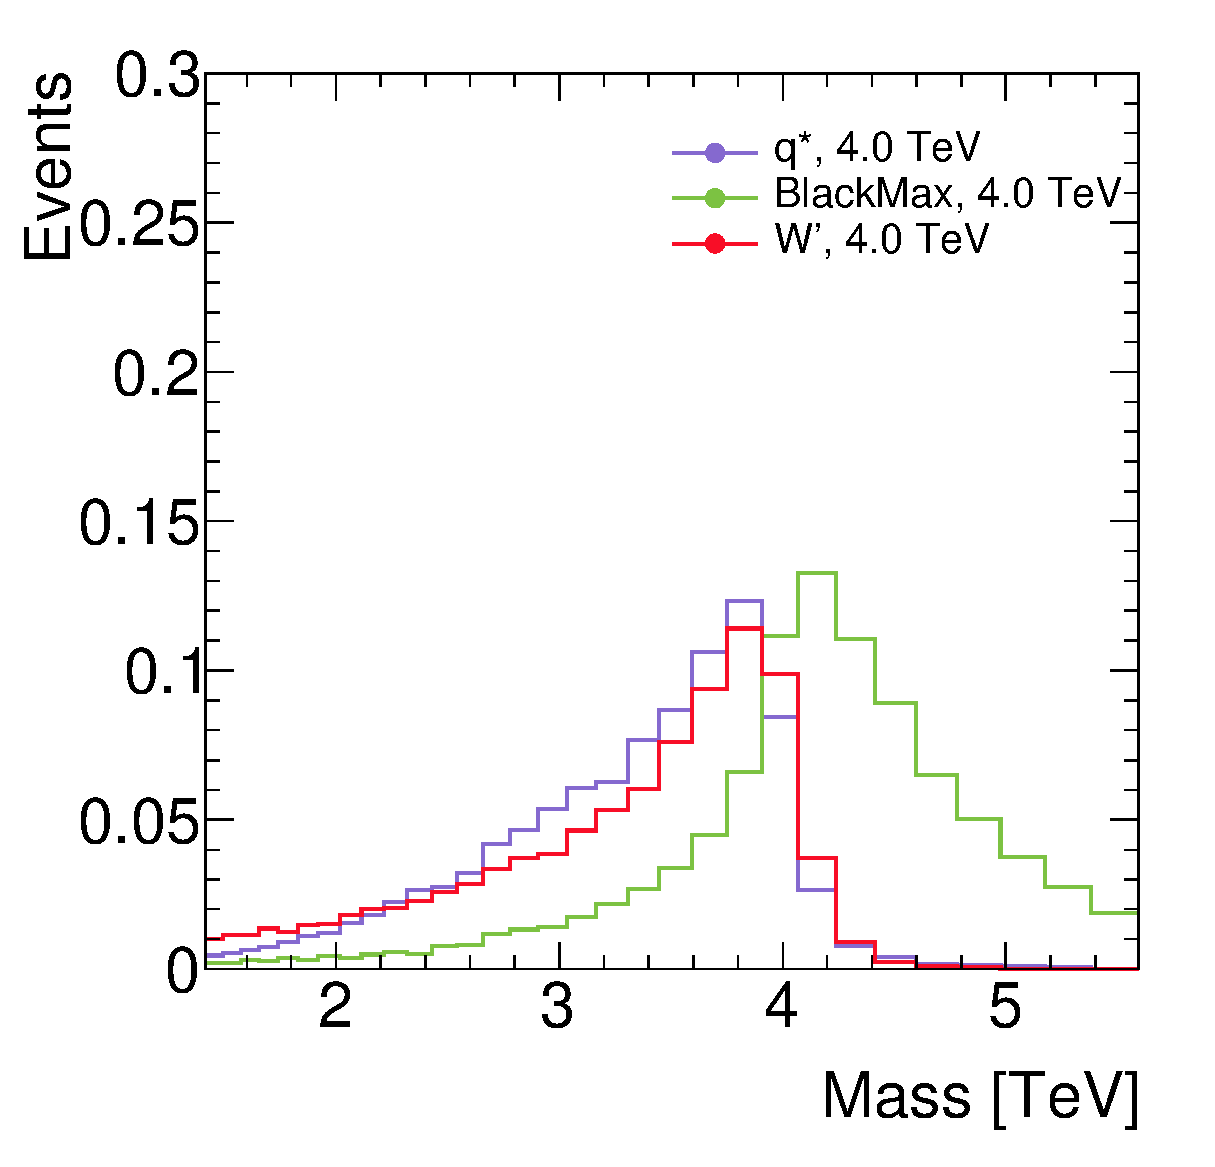
\includegraphics[width=0.45\textwidth]{figures/benchmark_signals/overlaidSignals_m4000_linear.eps}}
%\subfigure[6.5 TeV]{\label{fig:resonance_templates_6500}
%               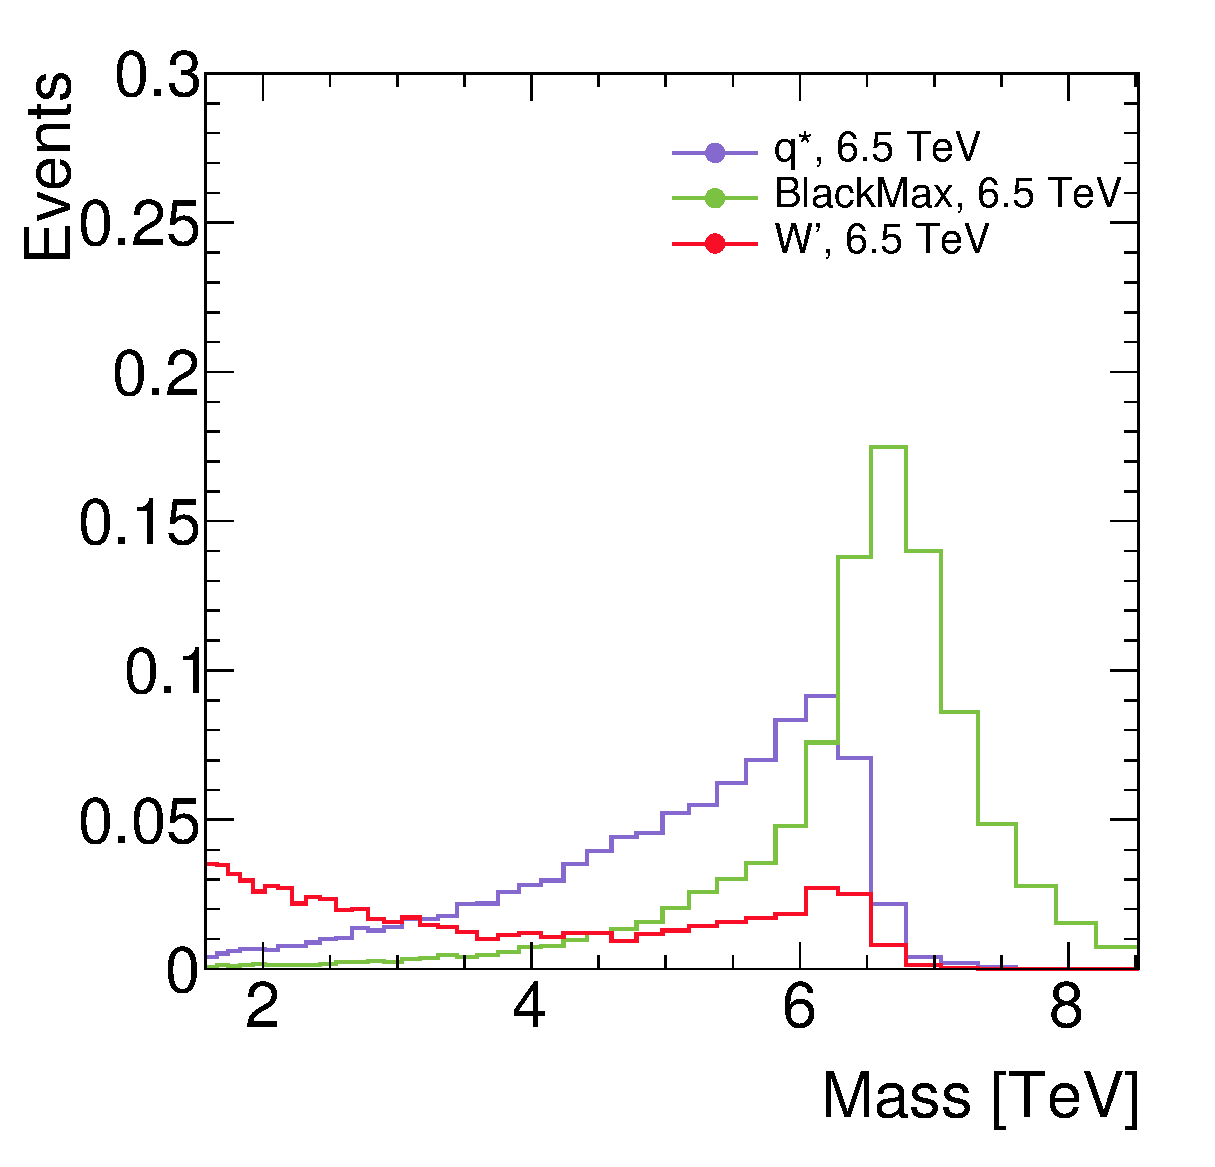
\includegraphics[width=0.45\textwidth]{figures/benchmark_signals/overlaidSignals_m6500_linear.eps}}
%\subfigure[4.0 TeV, truncated]{\label{fig:resonance_tr_templates_4000}
%               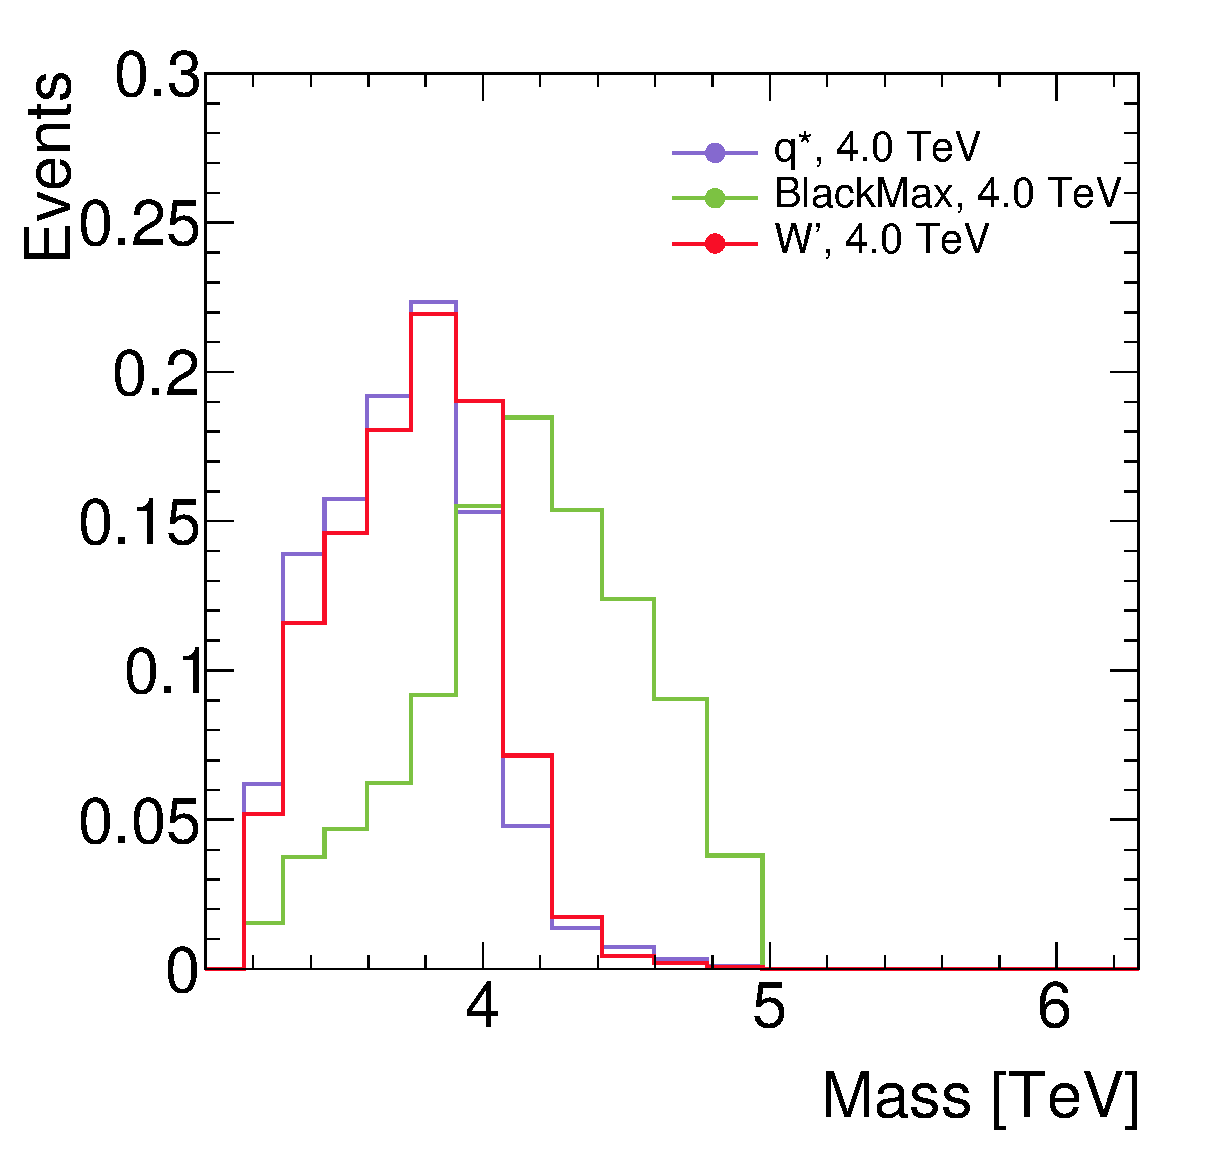
\includegraphics[width=0.45\textwidth]{figures/benchmark_signals/overlaidSignals_m4000_trunc.eps}}
%\subfigure[6.5 TeV, truncated]{\label{fig:resonance_tr_templates_6500}
%               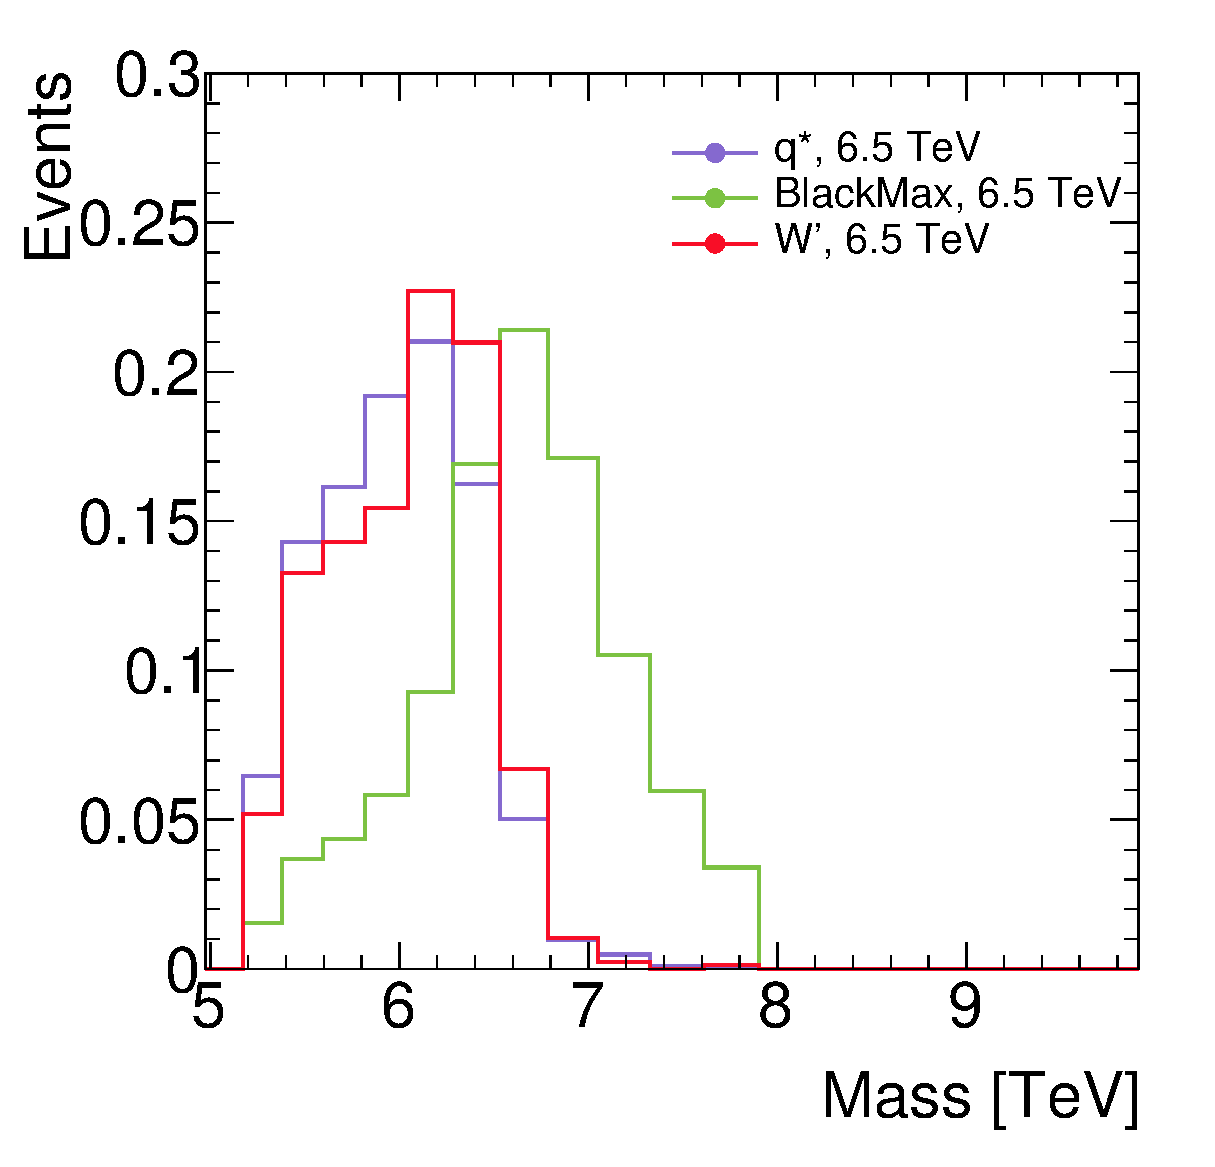
\includegraphics[width=0.45\textwidth]{figures/benchmark_signals/overlaidSignals_m6500_trunc.eps}}
%
%\caption{Normalized \mjj\ templates at 4.0 TeV \subref{fig:resonance_templates_4000},\subref{fig:resonance_tr_templates_4000} and 6.5 TeV \subref{fig:resonance_templates_6500},\subref{fig:resonance_tr_templates_6500}, before (above) and after (below) the truncation procedure, for various resonant benchmark models. The signals are re-normalised after truncation for ease of comparison of the shapes.}
%\label{fig:resonance_templates_shapes}
%\end{figure}
%

%\clearpage
%%%%%%%%%%%%%%%%%%%%%%%%%%%%%%%%%%%%%%%%%%%%%%%%%%%%%%%%%%%%%%%%%%%%
%\subsubsection{Signal Morphing}
%\label{sec:SwiftMorphing}
%%%%%%%%%%%%%%%%%%%%%%%%%%%%%%%%%%%%%%%%%%%%%%%%%%%%%%%%%%%%%%%%%%%%

%\todo[inline] {Will we use morphing?}


%Smooth signal mass distributions are obtained  from morphing the signal shapes from MC. The MC signals are fit to a Gaussian + reverse Landau function, a parameterization that has one normalization and five shape parameters. The parameters are interpolated as a function of mass using cubic splines. This allows the use of signal shapes at any mass. Figure~\ref{fig:morphing} shows some examples of fits to MC signal shapes as well as several interpolated signal shapes.  
%
%\begin{figure}[!htb]
%	\centering
%	\subfigure[q* signals]{ \includegraphics[width=0.48\textwidth]{figures/SWiFt/interpolate_qStar.pdf} }
%	\subfigure[Reclustered W' signals]{ \includegraphics[width=0.48\textwidth]{figures/SWiFt/interpolate_WPrimeRe.pdf} }
%	\subfigure[Z' 0.2 SM coupling signals]{ \includegraphics[width=0.48\textwidth]{figures/SWiFt/ZPrime_gSM0p20.pdf} }
%	\subfigure[Z' 0.5 SM coupling signals]{ \includegraphics[width=0.48\textwidth]{figures/SWiFt/ZPrime_gSM0p50.pdf} }
%	\caption{
%		Signal morphing for some MC signals. The solid colored histograms are MC signal shapes and the dotted lines of the same color are fit to the MC shapes. The dotted pink curves are the morphed shapes.  
%		\label{fig:morphing}}
%\end{figure}
%
%To stress test the morphing technique, tests were done where the a set of mass MC signal shapes were removed and the morphing was done with the remaining shapes. The results of this test is shown in figure~\ref{fig:morphingTest}, where in (a) integer MC q* shapes (2 \TeV\ , 3 \TeV\ , 4 \TeV\ , 5 \TeV\ , 6 \TeV\ ) are removed and morphing is done using the odd shapes only and in (b) fractional MC shapes (2.5 \TeV\ , 3.5 \TeV\ , 4.5 \TeV\ , 5.5 \TeV\ ) are removed and the even shapes are used for morphing. The technique recovers the shapes of the removed signals fairly well.  
%
%\begin{figure}[!htb]
%	\centering
%	\subfigure[q* signals. Morphing with odd masses only.]{ \includegraphics[width=0.48\textwidth]{figures/SWiFt/interpolateWorking_evenRemoved.pdf} }
%	\subfigure[q* signals. Morphing with even masses only.]{ \includegraphics[width=0.48\textwidth]{figures/SWiFt/interpolateWorking_oddRemoved.pdf} }
%	\caption{
%		Signal morphing stress test. (a) Even mass signals are removed and morphing is done with odd masses only. (b) Odd mass signals are removed and morphing is done with even masses only. 
%		\label{fig:morphingTest}}
%\end{figure}  
%


